Atunci când vorbim despre o aplicație ce propune crearea unui model acustic pentru simularea sunetului în încăperi este foarte important să ne ridicăm problema validării acestuia folosind de exemplu un software similar existent pe piață. În cadrul acestui studiu pentru a fi verificată corectitudine si validitatea acestui soft am realizat o serie de unit teste ce au fost prezentate în capitolul anterior și, mai mult de atât, am realizat o serie de comparații cu software-ul Simcenter 3D.

Simcenter 3D este o platformă de simulare complet integrată pentru modelarea, simularea și analizarea produselor și sistemelor complexe de inginerie. Platforma include soluții puternice de simulare pentru mai multe discipline, inclusiv analize structurale, acustice, de flux, termice, de mișcare și compozite, precum și optimizare și simulare multifizică. Software-ul își propune să permită simulărilor să joace un rol timpuriu în procesul de proiectare, ducând la creșterea calității, eficienței și inovației.

Pentru validarea modelului acustic am creat o cameră rectangulară, folosind ambele soft-uri, cu dimensiunile: 30m lățime, 30m lungime si 15m înălțime, unde am plasat sursa $S$ la poziția $S(0, 2.5,0)$, iar microfoanele au fost așezate astfel: 

\begin{itemize}
	\utb $M0(2, 1.6, 1.7)$, fiind la o distanța de 3.07m de sursă
	
	\utb $M1(-1.5, 1.2, 1.7)$, fiind la o distanța de 2.56m de sursă
	
	\utb $M2(1, 2, 13)$, fiind la o distanța de 13.19m de sursă
\end{itemize}

Similaritatea celor două camere se poate observa în Figura \ref{asemanatoare}.

Ambele software-uri permit crearea celor două încăperi, crearea unei surse audio și a unor microfoane statice, setarea numărului maxim de reflexii, setarea lungimii maxime a unei raze, setarea pasului de frecvență, folosirea unei melodii, setarea puterii. Diferența dintre cele două software-uri este că Simcenter nu permite setarea numărului de raze ce va fi distribuit în încăpere. Din acest motiv am încercat să găsim un echivalent pentru numărul de raze ce trebuie trasate în încăpere folosind modelul acustic propus de această lucrare. Configurația folosită va fi:

\begin{itemize}
	\utb 1 000 000 de raze distribuite uniform în cazul modelului acustic propus de această lucrare
	
	\utb maxim 10 reflexii pentru o rază
	
	\utb 200m distanța maximă pe care o rază o poate parcurge
	
	\utb 8192Hz rezoluția frecvenței
\end{itemize}

Numărul de raze obținut de modelul vizat de această lucrare este 1143, iar numărul de raze care ajunge pe microfonul $M2$ folosind Simcenter este 1400. Conform acestor configurații putem observa similaritatea rezultatelor obținute folosind ambele software-uri urmărind Figura \ref{fig:Fig25} și Figura \ref{fig:Fig26}.

\begin{figure}[!htb]%
	\begin{subfigure}[b]{.48\textwidth}
		\centering
		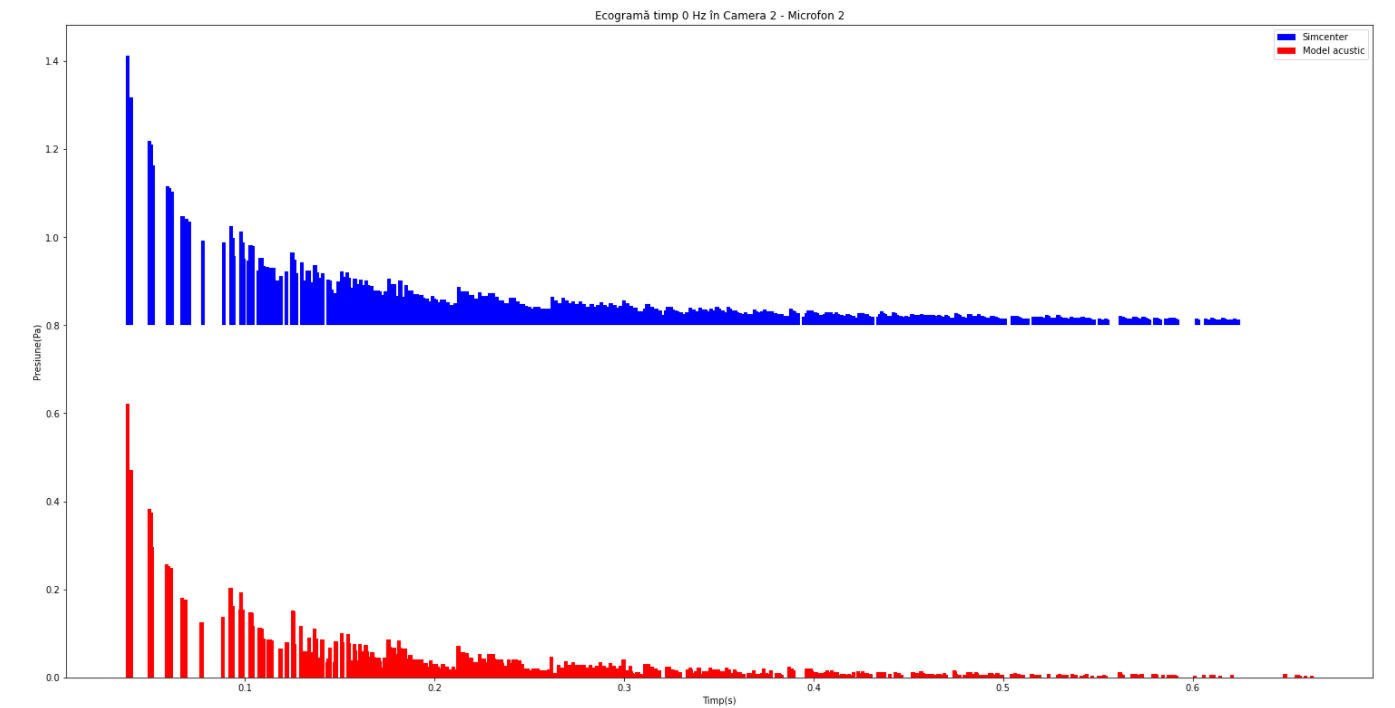
\includegraphics[width=1\linewidth]{imagini/eco_2.png} 
		\caption{Ecogramă timp }
		%\label{fig:sub-fig}
	\end{subfigure}
	\hfill
	\begin{subfigure}[b]{.48\textwidth}
		\centering
		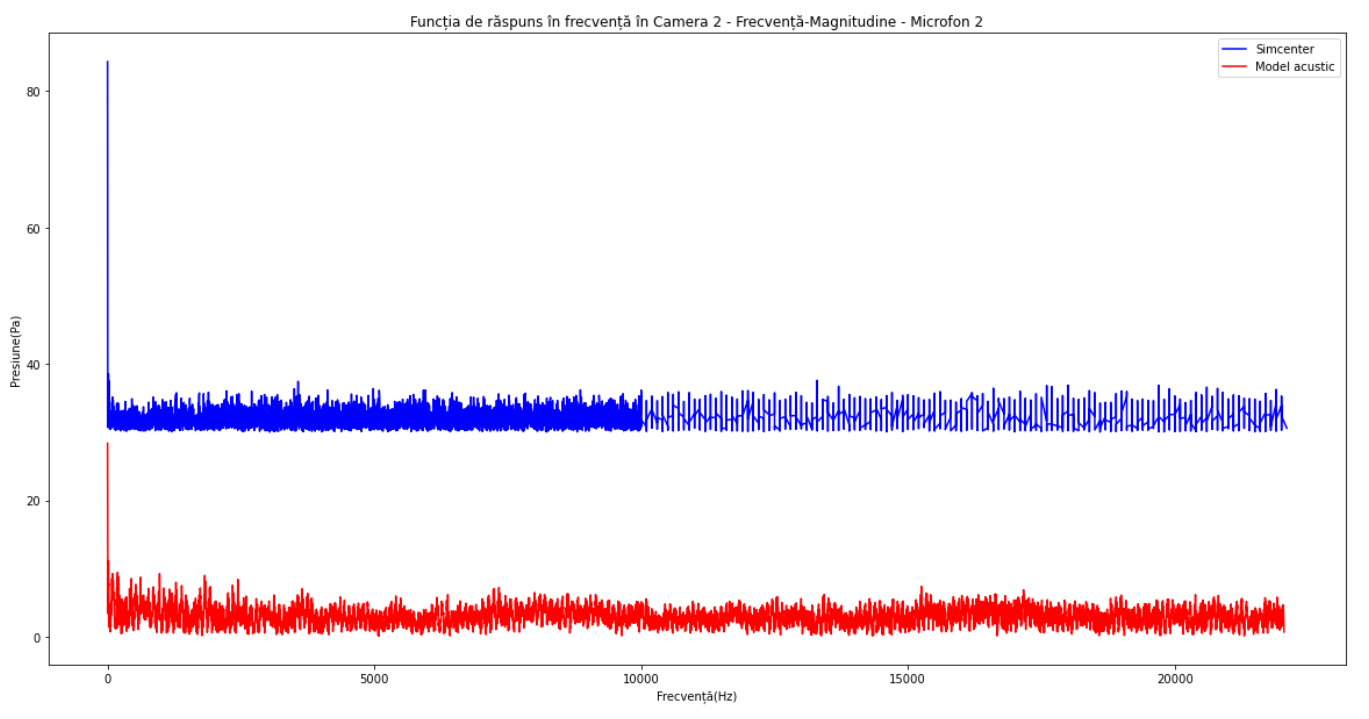
\includegraphics[width=1\linewidth]{imagini/ir_2.png}
		\caption{Funcția de răspuns la impuls}
		%\label{fig:sub-second}
	\end{subfigure}
	
	\caption{Ecogramă timp și funcția de răspuns la impuls pe microfonul $M2$ }
	\label{fig:Fig25}	
\end{figure}

\begin{figure}[!htb]%
	\begin{subfigure}[b]{.48\textwidth}
		\centering
		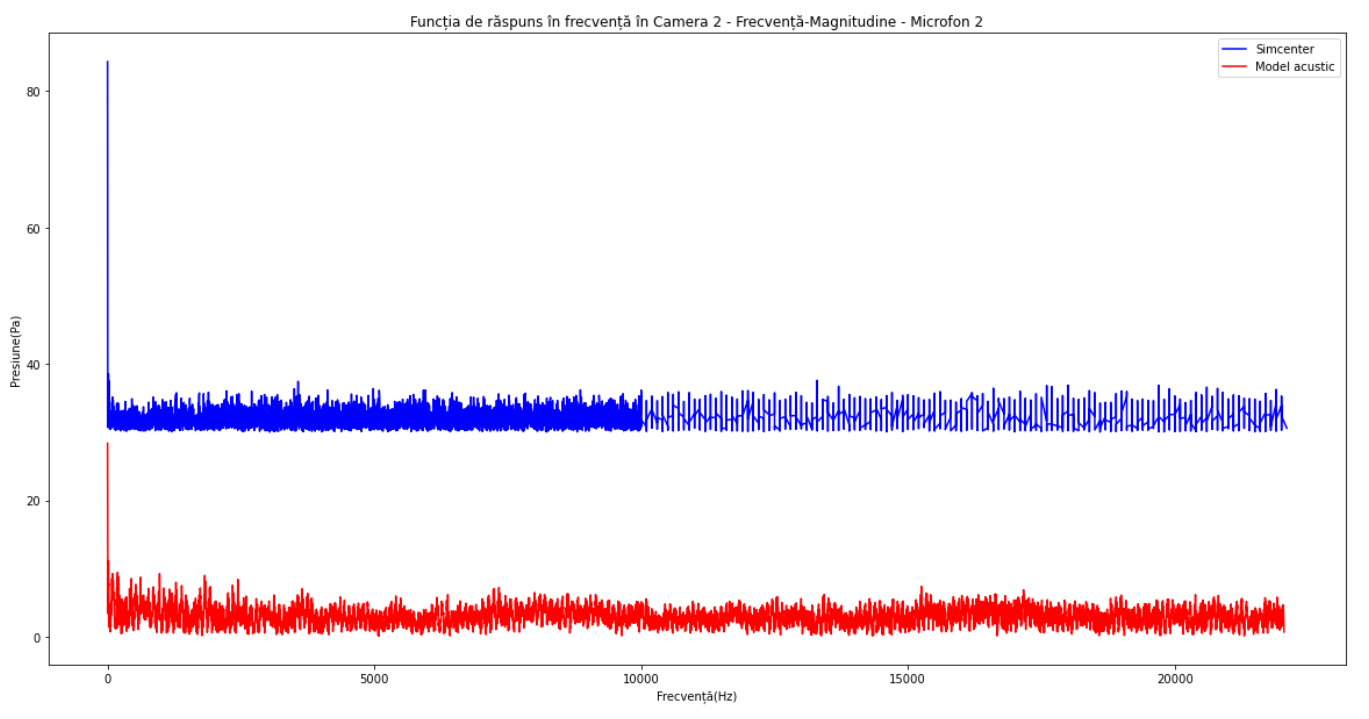
\includegraphics[width=1\linewidth]{imagini/ir_2.png} 
		\caption{Grafic Frecvență-Magnitudine}
		%\label{fig:sub-fig}
	\end{subfigure}
	\hfill
	\begin{subfigure}[b]{.48\textwidth}
		\centering
		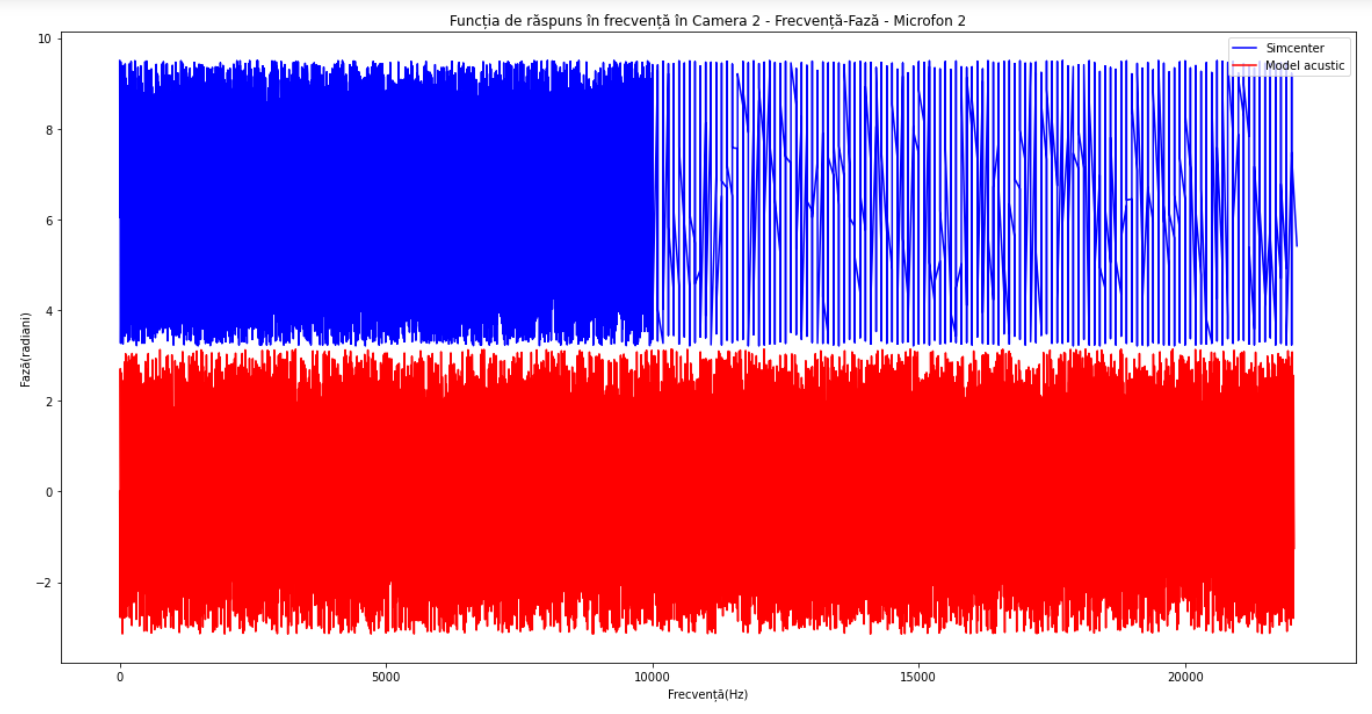
\includegraphics[width=1\linewidth]{imagini/ir_1_2.png}
		\caption{Grafic Frecvență-Fază}
		%\label{fig:sub-second}
	\end{subfigure}
	
	\caption{Funcția de răspuns în frecvență pe microfonul $M2$}
	\label{fig:Fig26}	
\end{figure}